\documentclass[a4paper, 12pt]{article}
\usepackage{arxiv}
\usepackage[T2A]{fontenc}
\usepackage[utf8]{inputenc}
\usepackage[english, russian]{babel}
\usepackage{url}
\usepackage{booktabs}
\usepackage{amsfonts}
\usepackage{nicefrac}
\usepackage{microtype}
\usepackage{lipsum}
\usepackage{graphicx}
\usepackage{natbib}
\usepackage{doi}
\usepackage{amsthm}

\usepackage[utf8]{inputenc}
\usepackage{amsmath}
\usepackage{mathtools}
\usepackage{extsizes} % Возможность сделать 14-й шрифт
\newtheorem{theorem}{Теорема}
% \renewcommand{\shorttitle}{\textit{arXiv} Template}
\renewcommand{\headeright}{}
\renewcommand{\undertitle}{}
\renewcommand{\abstractname}{Аннотация}
\newcommand{\keywordsname}{Ключевые слова:}

\begin{document}
\title{Выбор интерпретируемых рекуррентных моделей глубокого обучения}
\author{\normalsize\bf{Гапонов Максим,~Бахтеев Олег,~Яковлев Константин,~Стрижов Вадим} \\
	Московский физико-технический институт \\
	\texttt{\{gaponov.me,~bakhteev,~...,~strijov\}@phystech.edu}
}
\date{}
\maketitle
\begin{abstract}
Рассматривается задача интерпретации рекуррентных нейронных сетей. Под интерпретируемостью модели понимается возможность получить простую зависимость выходных данных от входных. Интерпретируемость нейронных сетей необходима для повышения уровня доверия к предсказаниям таких моделей. Предлагается обобщить метод OpenBox, предназначенный для интерпретации нейронных сетей с кусочно-линейными функциями активации. Нейронная сеть представляется в виде набора интерпретируемых линейных классификаторов. Каждый из классификаторов определён на выпуклом многограннике. Поэтому интерпретации близких объектов оказываются согласованными. Для проверки работоспособности предложенного метода проводится эксперимент на выборке IMDB Review dataset.
\end{abstract}

\keywords{Интерпретация моделей \and Рекуррентные нейронные сети \and Кусочно-линейные модели}

\section{Введение}
В работе рассматривается метод интерпретации рекуррентных моделей глубокого обучения. Такие модели используются для обработки последовательностей данных \cite{lipton2015critical}. Однако для принятия решения при помощи такой модели необходимо доверять её предсказаниям. По этой причине требуется построить интерпретируемую модель, объясняющую предсказания исходной модели. Работа посвящена построению и выбору таких интерпретируемых моделей для некоторого класса рекуррентных сетей.

Рекуррентная нейронная сеть представляет из себя последовательность из слоёв нейронов: входного слоя, скрытых слоёв и выходного слоя \cite{sherstinsky2020fundrnn}. Отличительной особенностью от обыкновенных нейронных сетей являются циклические связи между нейронами. Такие связи позволяют запоминать состояния для обработки последовательностей данных.

Интерпретация должна быть \textbf{точной} и \textbf{согласованной} \cite{chu2019exact}. Интерпретация называется точной, если она согласуется с поведением модели. То есть показывает значимыми те признаки, которые значимо повлияли на предсказание модели. Интерпретация называется согласованной, если интерпретации близких объектов похожи. То есть значимости признаков отличаются незначительно.

Анализ зависимости предсказания модели от входных данных в реккурентных нейронных сетях является сложной задачей. Методы, рассмотренные в работах \cite{dosovitskiy2016inverting, zhou2018interpreting, NIPS2014_ea8fcd92, bastani2019interpreting, zhou2015learning, simonyan2014deep} являются либо неточными, то есть не отвечают реальному поведению модели, либо несогласованными, то есть совершенно разным образом объясняет предсказания на близких объектах.

В работах \cite{dosovitskiy2016inverting, zhou2018interpreting} рассмотрены методы, основанные на интерпретации признаков, выученных скрытыми слоями. Такой подход отражает поведение скрытых слоёв, но не показывает поведение сети в целом. В работах \cite{NIPS2014_ea8fcd92, bastani2019interpreting} предлагаются методы подражания модели. В этом подходе строится модель с похожим на исходную поведением. Построенная модель имеет более простую структуру, поэтому проще интерпретируется. Однако из-за недостаточно сложной структуры построенная модель недостаточно хорошо приближает исходную. Наконец, в работах \cite{zhou2015learning, simonyan2014deep} рассмотрены методы локальной интерпретации, в которых происходит анализ поведения модели в окрестности исходного объекта. В таком подходе получается точная интерпретация одного объекта, однако интерпретации близких объектов могут существенно отличаться. Таким образом, данный подход не предоставляет согласованные интерпретации.

Рассмотренный в данной работе подход является обобщением метода OpenBox для интерпретации нейронных сетей с кусочно-линейными  функциями активации \cite{chu2019exact}. Нейронная сеть представляется в виде эквивалентного набора линейных классификаторов. Каждый из них классифицирует объекты внутри некоторого выпуклого многогранника в пространстве признаков, поэтому интерпретации получаются согласованными.

На выборке IMDB Movie Review Dataset \cite{maas-EtAl:2011:ACL-HLT2011} проведён вычислительный эксперимент для анализа качества метода, а также для проверки интерпретаций на точность и согласованность. 

\section{Постановка задачи}
Рассмотрим рекуррентную нейронную сеть $\mathbf{f}$ с кусочно-линейными функциями активации. Входные данные обозначим через $\mathbf{x} \in \mathbf{X}$, где $\mathbf{X} \subset \mathbb{R}^d$ --- пространство признаков. Предсказание модели $\mathbf{f}$ обозначим через $\mathbf{y} \in \mathbf{Y}$, где $\mathbf{Y}$ --- пространство предсказаний.

Модель представляет из себя функцию классификации $\mathbf{f}: \mathbf{X} \to \mathbf{Y}$. Из-за сложной структуры сети трудно интерпретировать поведение функции $\mathbf{f}$, поэтому необходимо получить интерпретацию, которую способен понять человек.

Требуется построить модель, соответствующую функции $\mathbf{g}$, которая обладает следующими свойствами.

Во-первых модель должна быть интерпретируемой. То есть можно построить простую зависимость выходных данных от входных (интерпретацию). Также модель должна быть точной, то есть функции $\mathbf{f}$ и $\mathbf{g}$ должны совпадать на множестве $\mathbf{X}$. Помимо этого, модель должна быть согласованной, то есть интерпретации близких объектов в пространстве $\mathbf{X}$ должны быть похожи.

% Функция $F$ является кусочно-линейной, так как $\mathbf{N}~-$ рекуррентная нейронная сеть с кусочно-линейными функциями активации. Области, на которых функция $F$ линейна являются выпуклыми многогранниками.

% Предлагается рассмотреть модель $\mathbf{M}$, представляющую из себя множество линейных классификаторов $\left\{F_1, F_2, \dots, F_h, \dots\right\}$. Пространство признаков $\mathbf{X}$ разбивается на конечное множество выпуклых многогранников $\left\{P_1, P_2, \dots, P_h, \dots\right\}$. То есть $\bigsqcup\limits_{h} P_h=\mathbf{X}$. Классификатор $F_h$ определён на многограннике $P_h$. Модель $\mathbf{M}$ должна быть математически эквивалентна модели $\mathbf{N}$, то есть множество функций $\left\{F_1, F_2, \dots, F_h, \dots\right\}$ определённых на $\left\{P_1, P_2, \dots, P_h, \dots\right\}$ тождественно равно функции $F$, определённой на $\mathbf{X}$.

% Модель $\mathbf{M}$ обладает свойством точности, так как математически эквивалентна модели $\mathbf{N}$. То есть поведение двух моделей совпадает. $F|_{P_h} \equiv F_h$. Модель $\mathbf{M}$ также обладает свойством согласованности, так как близкие объекты попадают в один и тот же выпуклый многогранник $P_h$, а значит, классифицируются одним и тем же линейным классификатором $F_h$.

%Задача состоит в поиске такой модели $\mathbf{M}$, построении множества классификаторов по произвольной рекуррентной нейронной сети $\mathbf{N}$.

\section{Вычислительный эксперимент}

В рамках эксперимента рассматривается задача классификации отзывов на ресурсе IMDB. Используется выборка IMDB Movie Review Dataset \cite{maas-EtAl:2011:ACL-HLT2011} состоящяя из 50 000 отзывов, а также типов отзывов: положительный, отрицательный. Требуется по тексту отзыва определить вероятность принадлежности отзыва к классу положительных и отрицательных.

Для решения задачи используется рекуррентная нейронная сеть (обозначим через $\mathbf{f}$), принимающая векторы, полученные методом One-Hot Encoding \cite{onehot2018}. Рассматриваемая модель имеет 2 592 105 параметров. Такую модель нельзя считать легко интерпретируемой.

Выборка разделена на две части: тренировочную и тестовую. Модель обучается на тренировочной выборке. После обучения измеряется качество модели на тестовой выборке. Была получена точность классификации (доля верных ответов) около 60\%.

Интерпретацию модели $\mathbf{f}$ будем производить при помощи метода LIME \cite{ribeiro2016why}. Для построения интерпретации предсказания объекта $\mathbf{x}$ строится линейная модель $\mathbf{g}$ с небольшим числом параметров (число параметров обозначим через $K$), которая приближает поведение модели $\mathbf{f}$ в окрестности объекта $\mathbf{x}$. Для этого порождаются новые объекты $\mathbf{x_1}, \mathbf{x_2}, \dots, \mathbf{x_n}$ в окрестности объекта $\mathbf{x}$. Вычисляются предсказания $\mathbf{y_1}, \mathbf{y_2}, \dots, \mathbf{y_n}$ модели $\mathbf{f}$ на объектах $\mathbf{x_1}, \mathbf{x_2}, \dots, \mathbf{x_n}$. То есть $\mathbf{y_i}=\mathbf{f}(\mathbf{x_i})$.

Линейная модель $\mathbf{g}$ с $K$ параметрами строится таким образом, чтобы как можно точнее классифицировать объекты $\mathbf{x_1}, \mathbf{x_2}, \dots, \mathbf{x_n}$ с истинными метками $\mathbf{y_1}, \mathbf{y_2}, \dots, \mathbf{y_n}$. Интерпретацией в данном случае являются веса исходных признаков, а именно присутствия/отсутствия слов в отзыве.

\section{Результаты эксперимента}

Предсказание полученной методом LIME выглядит следующим образом.

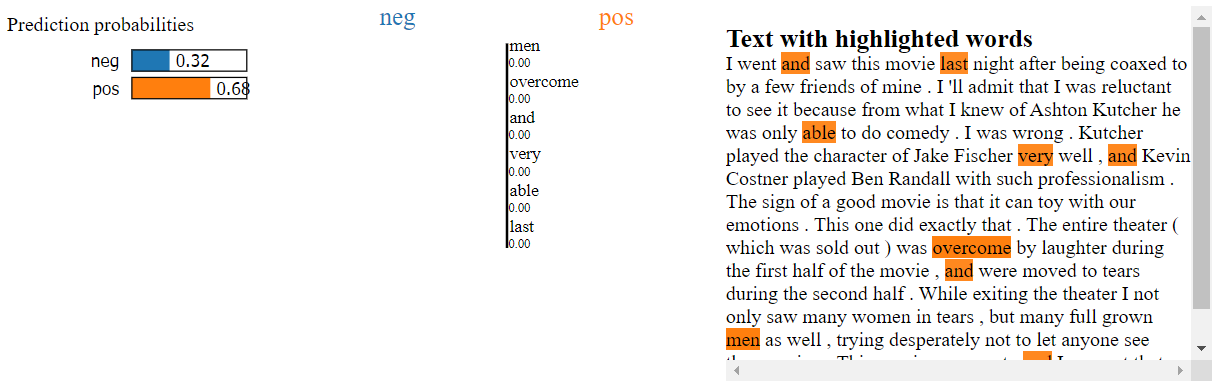
\includegraphics[width=\textwidth]{figures/lime_exp.png}

Подсвеченные слова сильнее всего влияют на результат. Как можно заметить, модель отнесла отзыв к положительному классу, основываясь на наличии слов \texttt{and, able, men, last}. Понятно, что данные слова одинаково часто могут появиться как в положительном отзыве, так и в отрицательном. Таким образом, даже не учитывая метрику accuracy модели, можно сделать вывод, что модель непригодна для использования, так как делает предсказания на основе нерелевантных признаков. Однако из-за особенностей выборки непригодность модели можно не заметить, если рассматривать только метрики качества. 

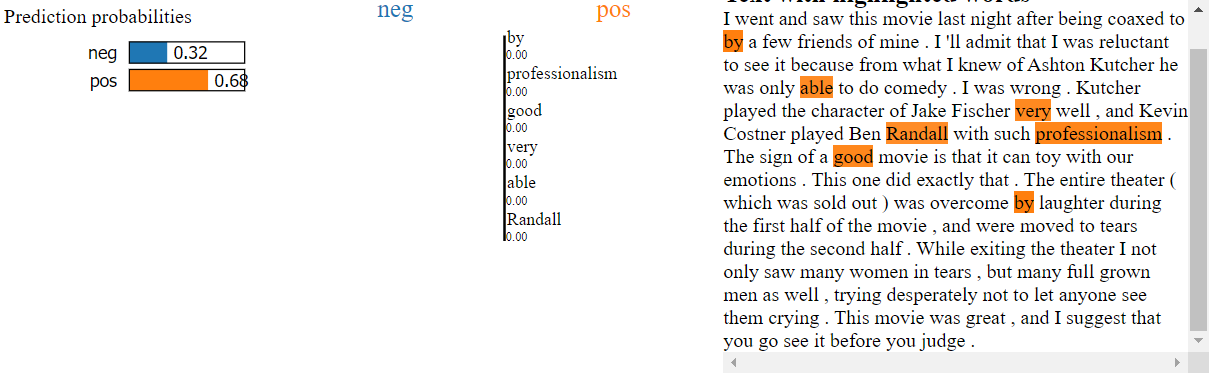
\includegraphics[width=\textwidth]{figures/lime_exp2.png}

Вторая картинка показывает нам, что интерпретации несогласованны. А именно, значимые слова сильно отличаются. Такой эффект может быть связан с высокой сложностью модели.

Также можно отметить, что метод LIME является не самым эффективным методом с точки зрения времени.

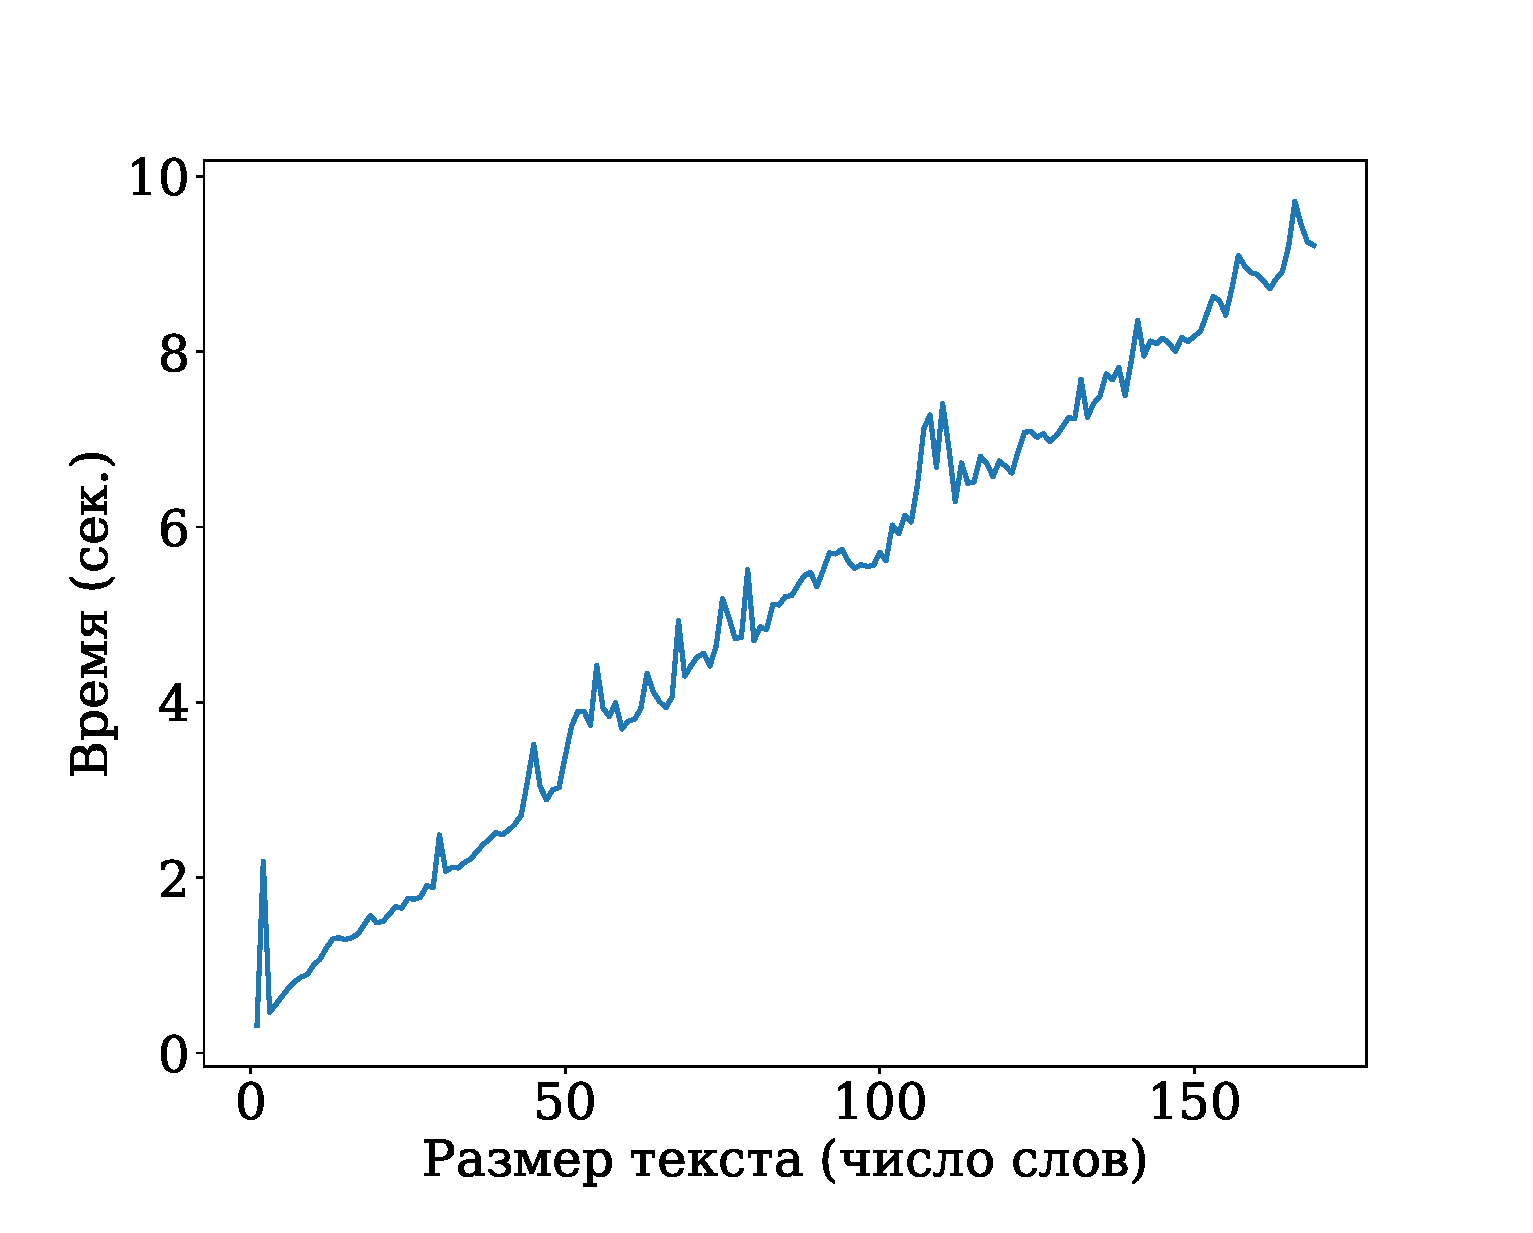
\includegraphics[scale=0.5]{../figures/lime_time}

Как видно из графика, на данной модели метод LIME способен обработать около 20 слов в секунду.

Вышеперечисленных недостатков мы постараемся избежать в новом подходе.

Для оценки качества интерпретации требуется построить следующие графики:
\begin{itemize}
\item Распределение предсказаний интерпретируемой модели

\item Косинусное расстояние между предсказаниями исходной модели и построенной интерпретируемой модели
\end{itemize}

\section{Интерпретация рекуррентных нейронных сетей}

Рассмотрим рекуррентную нейронную сеть $\mathbf{N}$. Её можно представить в виде обыкновенной нейронной сети, заменив рекуррентные слои на последовательность обыкновенных слоёв нейронов. А именно, пусть дан слой рекуррентной нейронной сети состоящий из $n$ нейронов с кусочно-линейной функцией активации $f$. Обозначим число рекуррентных запусков данного слоя через $k$. Заменим в архитектуре нейронной сети данный слой на $k$ слоёв, состоящих из $n$ нейронов, с функциями активации $f$. Таким образом, нейронная сеть представляется в виде обыкновенной сети.

Введём обозначения.

$L~-$ число слоёв нейронной сети

$\mathbf{x}_0~-$ исходный объект

$\mathbf{a}_i~-$ вход слоя с номером $i$

$f_i~-$ функция активации после слоя с номером $i$

$\mathbf{W}_i~-$ матрица линейного преобразования слоя с номером $i$

$\mathbf{b}_i~-$ вектор сдвига

$$a_i=f_i\left(\mathbf{W}_i \mathbf{a}_{i} + \mathbf{b}_i\right)$$

$$\mathbf{a}_1=\mathbf{x}_0$$

Рассматриваются кусочно-линейные функции активации, то есть

\[f(x)=\left\{
\begin{array}{ll}
      r_1 x+t_1 & \text{if } x\in I_1 \\
      r_2 x+t_2 & \text{if } x\in I_2 \\
      \dots&\dots\\
      r_u x+t_u & \text{if } x\in I_u \\
\end{array} 
\right. \]

Причём $I_1,\dots,I_u$ - набор непересекающихся интервалов, покрывающий $\mathbb{R}$.

Для фиксированного исходного объекта $\mathbf{x}_0$ каждая кусочно-линейная функция $f_i$ является линейной в некоторой окрестности своего аргумента, то есть в окрестности $\mathbf{W}_i \mathbf{a}_{i} + \mathbf{b}_i$.

Также условие принадлежности аргумента $x$ интервалу $I_i~-$ это неравенство вида $p \leq x \leq q$.

\begin{theorem}
Пусть дана нейронная сеть $\mathbf{N}$ с кусочно-линейными функциями активации $f_i$. Тогда её можно представить в виде набора линейных функций $F_1,\dots,F_n$, каждая из которых определена на выпуклом многограннике $P_1,\dots,P_n$ в пространстве признаков $\mathcal{X}$.
\end{theorem}
\begin{proof}
Рассмотрим произвольный $\mathbf{x}_0\in\mathcal{X}$. Как уже было показано, кусочно-линейные функции активации $f_i$ являются линейными в некоторой окрестности своего аргумента, соответствующему $\mathbf{x}_0$. Причём условие принадлежности аргумента функции $f_i$ к интервалу $I_j~-$ это пересечение двух линейных неравенств. Каждое из неравенств задаёт полупространство в пространстве $\mathcal{X}$. Пересечение полупространств является выпуклым многогранником. Помимо этого, суперпозиция линейных функций является линейной функцией.

Таким образом, найден выпуклый многогранник $P_h$ и линейная функция $F_h$, заданная на этом многограннике и равная предсказаниям нейронной сети $\mathbf{N}$ на нём.

В силу произвольности выбора $\mathbf{x}_0$ получаем, что всё пространство $\mathcal{X}$ разбивается на выпуклые многогранники $P_h$, на которых заданы линейные функции $F_h$.

Нейронная сеть $\mathbf{N}$ имеет конечное число нейронов, значит, имеется конечное число неравенств, задающих полупространтва в пространстве $\mathcal{X}$. А конечное число неравенств задает лишь конечное число выпуклых многогранников. 
\end{proof}

Для решения задачи интерпретации рекуррентных нейронных сетей с кусочно-линейными функциями активации предлагается следующим алгоритм.

1. Вычислить коэффициенты линейного классификатора $F_h$, ($h$ такое, что $\mathbf{x}_0\in P_h$).

2. Выделить линейные неравенства на $\mathbf{x}_0$, соответствующие выпуклому многограннику $P_h$.

3. Интерпретацией модели на входном объекте $\mathbf{x}_0$ является набор коэффициентов линейного классификатора $F_h$, соответствующие им признаки, а также набор условий задающих $P_h$.

\section{Анализ ошибки}
На подвыборке размера 1000 объектов для каждого объекта найдём ближайший к нему. За меру близости возьмём коэффициент Жаккара. Построим интерпретацию на текущем объекте и предскажем вероятность принадлежности к положительному классу для ближайшего объекта. Чем меньше эта вероятность отличается от вероятности, которую предсказывает исходная модель, тем лучше. 

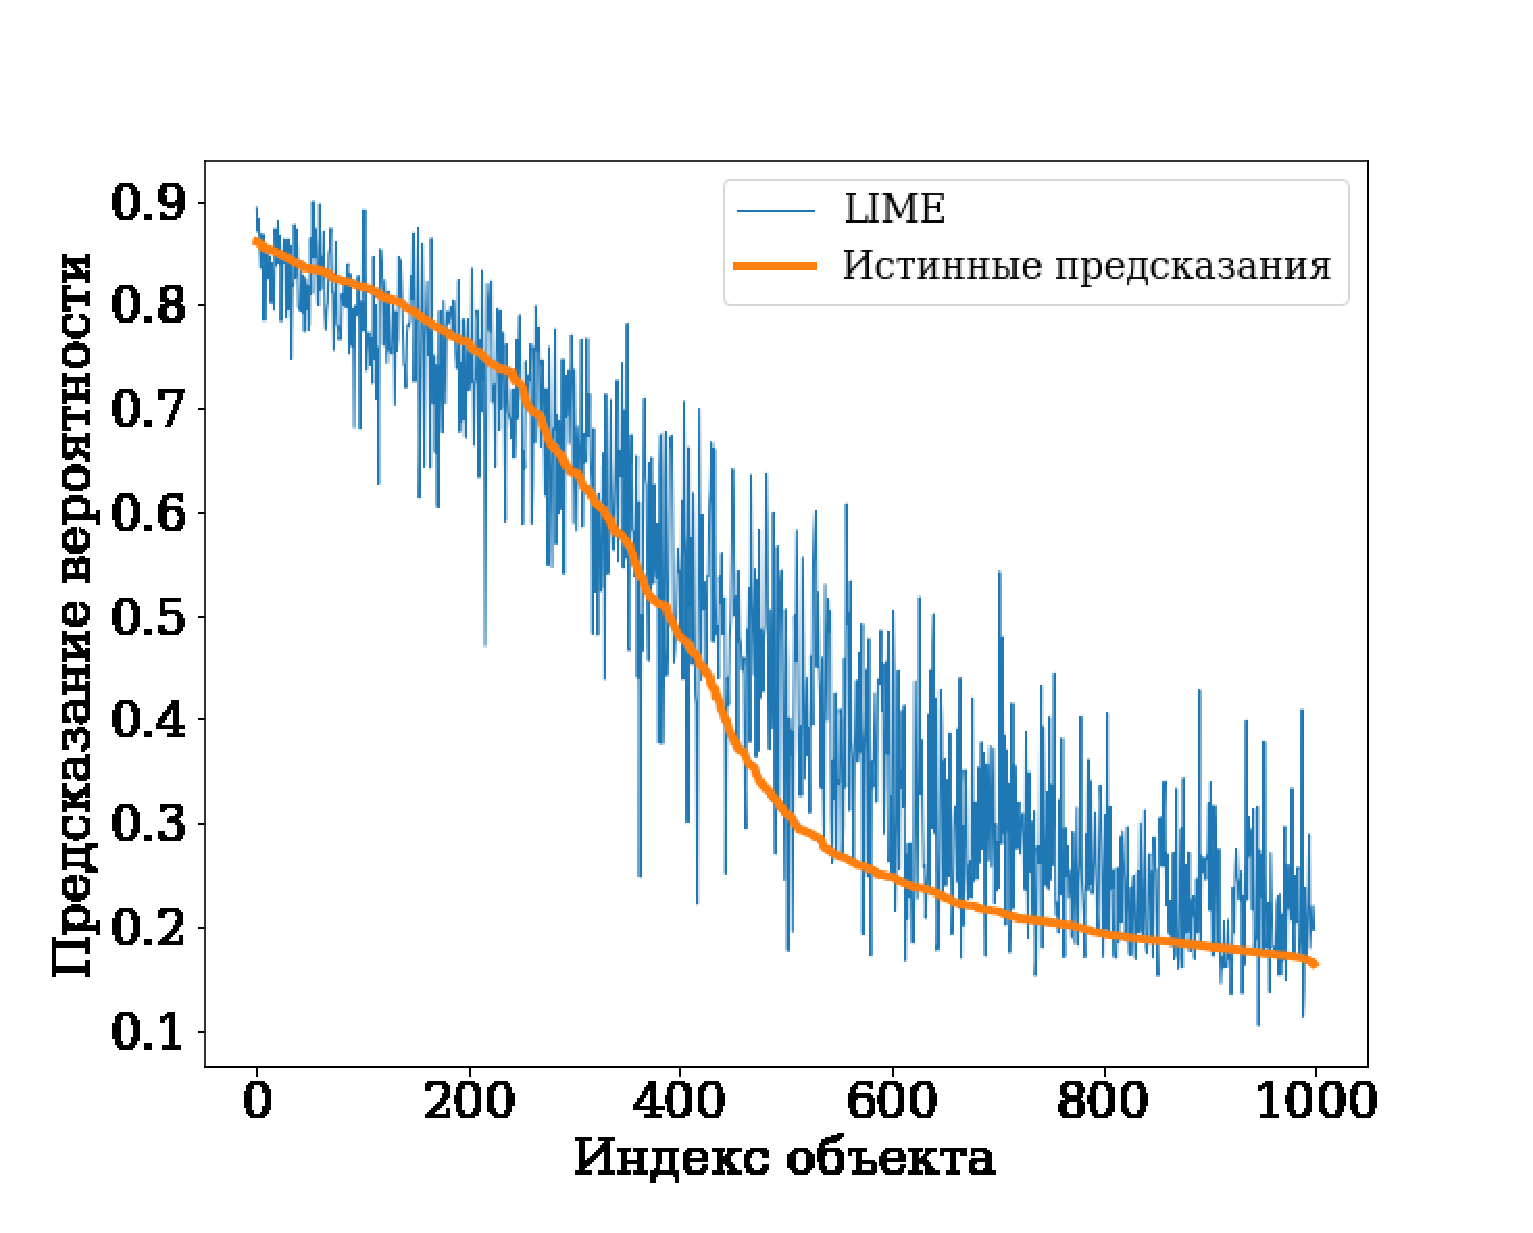
\includegraphics[width=0.9\textwidth]{../figures/lime_proba.eps}

Как видно из графика, метод LIME неточно предсказывает вероятность. График получился шумным и значительно отличается от истинных предсказаний. Преимущество метода OpenBox заключается в том, что полученная интерпретируемая модель оказывается математически эквивалентна исходной, то есть предсказания построенной модели равны предсказаниям исходной.

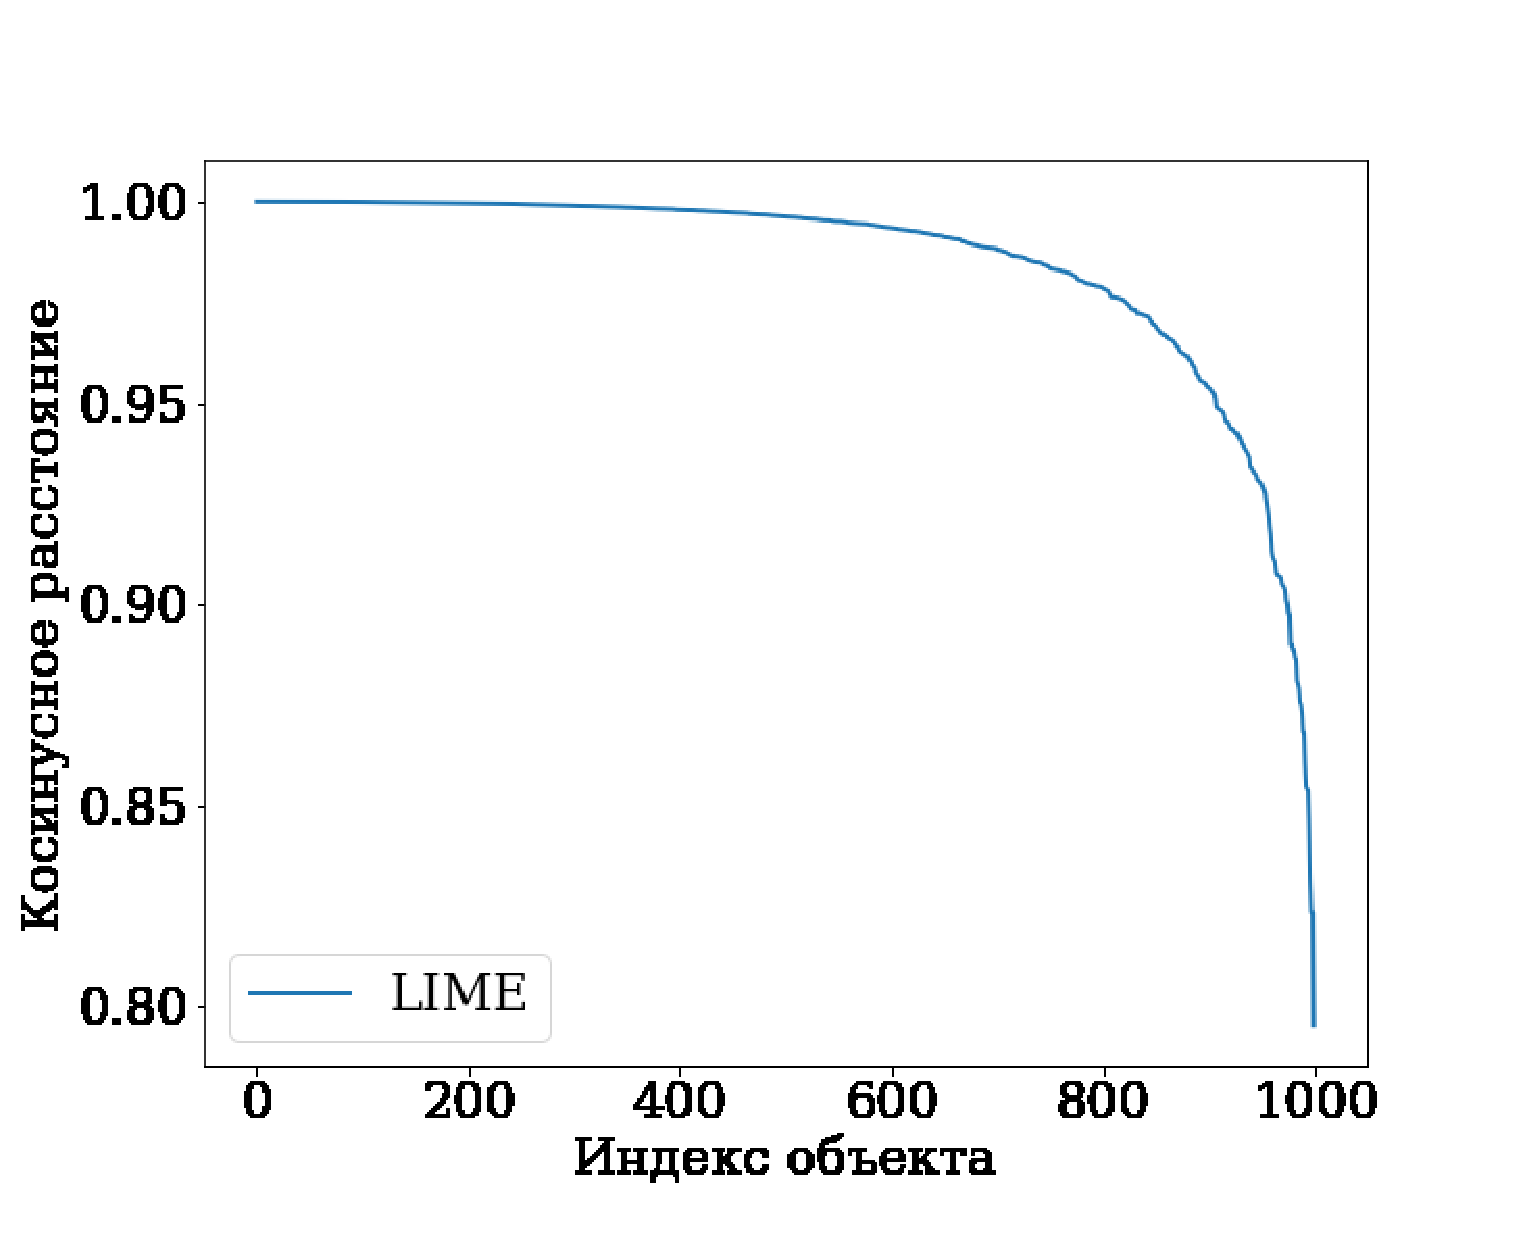
\includegraphics[width=0.9\textwidth]{../figures/lime_cosine.eps}

Как видно из следующего графика, предсказания, полученные методом LIME, для значительной доли объектов отличается с точки зрения косинусного коэффициента. Это значит, что для значительной доли объектов интерпретируемые предсказания не соответствуют истинным предсказаниям.

\bibliographystyle{unsrt}
\bibliography{Gaponov2022InterpretableRNN}

\end{document}
